\documentclass[12pt,letterpaper,noanswers]{exam}
\usepackage[usenames,dvipsnames,svgnames,table]{xcolor}
\usepackage[margin=0.9in]{geometry}
\renewcommand{\familydefault}{\sfdefault}
\usepackage{multicol}
\pagestyle{head}
\header{AM 111 Class 03}{}{Linear least squares, p.\thepage}
\runningheadrule
\headrule
\usepackage{siunitx}
\usepackage{graphicx} % more modern
\usepackage{amsmath} 
\usepackage{amssymb} 
\usepackage{hyperref}
\usepackage{tcolorbox}
\usepackage{enumitem}
\newcommand{\vc}[1]{\boldsymbol{#1}}
\DeclareMathOperator*{\argmin}{arg\,min} % thin space, limits underneath in displays

\begin{document}
 \pdfpageheight 11in 
  \pdfpagewidth 8.5in

\noindent 



\section{Preliminaries}
\begin{itemize}
\itemsep0pt
\item Problem set 01 is due on Friday at 5pm (submit via Gradescope and upload any source code to Canvas).
\item There will be a skill check in class during Class 04.  The problem info is below.
\item OH today 1-3pm and 4:30-6:30pm in Pierce G11 (AM Undergraduate Lounge).  Find all OH on Canvas.
\item Use Ed (find the link on Canvas) for questions about the problem set.
\end{itemize}



\noindent\textbf{Big picture}

Today: We will learn about way to compress data by describing a large dataset using just a few numbers.

\vspace{0.2cm}
\hrule
\vspace{0.2cm}

\noindent \textbf{Skill check practice}

Using $\left\{(x_i,y_i)\right\}_{i=1}^2 = \left\{(1,7), (2,4)\right\}$ as your data, and $f(x) = x^2$ as your model, 
\begin{parts}
\item construct the error vector $\vc{e}$, and
\item find the $1$-norm of $\vc{e}$
\end{parts}

\emph{You may be asked for the $1$-norm, $2$-norm, or $\infty$-norm of $\vc{e}$.}



\vspace{0.2cm}
\hrule
\vspace{0.2cm}

\noindent \textbf{Skill check solution}

$f(x_1) = 1^2 = 1$, $f(x_2) = 2^2 = 4$.  $\vc{e} = (7-1, 4-4) = (6,0)$.

The $1$-norm is $\vert 6\vert + \vert 0 \vert = 6.$
\vspace{0.2cm}
\hrule
\vspace{0.2cm}

\noindent \textbf{Teams}

\begin{multicols}{3}
1) Kevin, Eli, Daniyal

2) Caitlin, Julia, Johan

3) Ibrahima, Mai, Zachary

4) Sophie, Julia, Aidan

5) RJ, Brian, Nina

6) Kevin, Mack, Ray

7) Alex, Jack, Robert

8) Nini, Emma, Benjamin

9) Eletria, Tom, Basil

10) Jessica, Sandra, Padraig

11) Shang, Esmé, Marissa

12) Eric, Cameron, Dani

13) Alex, Ivonne, Mina
\end{multicols}


\section{Function fitting}
\noindent See Sauer chapter 4, Heath chapter 3, Greenbaum and Chartier chapter 7, Koumoutsakos notes from ETH lecture 1.

\vspace{0.1cm}

\subsection{Representing data}

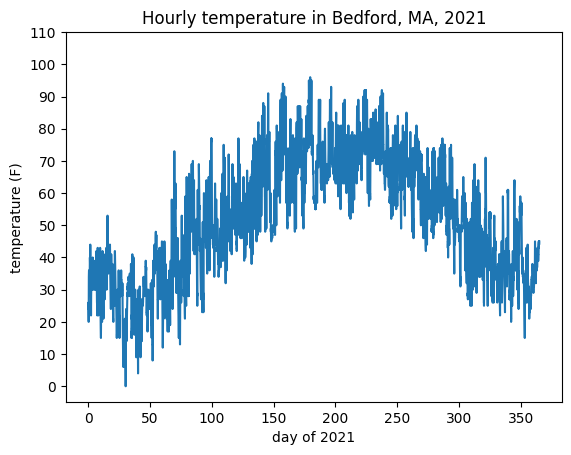
\includegraphics[width=0.45\linewidth]{img/C03weatherBedford.png}
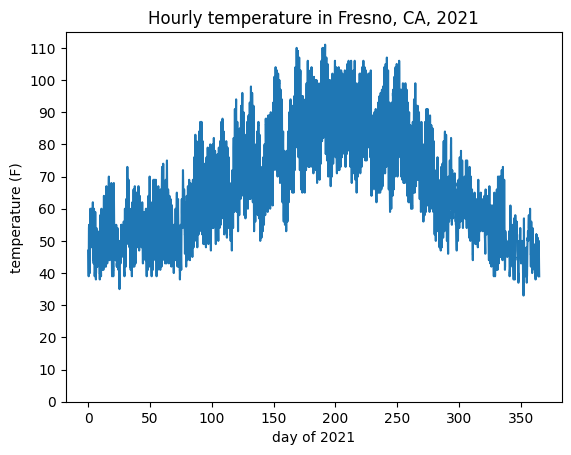
\includegraphics[width=0.45\linewidth]{img/C03weatherFresno.png}

NOAA NCEI data

\begin{enumerate}[series=classQ]
\item How would you summarize the Bedford data with a single number?  What about the Fresno data?

\emph{Have one member of your team use PollEverywhere \url{http://pollev.com/apmth111} to share your thoughts}

\item What if you could use two or three numbers?  How would you summarize each dataset?
\end{enumerate}
\vspace{1cm}

\noindent\textbf{Lower dimensional representations}
\begin{tcolorbox}
What is the typical temperature in Boston?
\begin{itemize}
\itemsep0pt
    \item approximating an ensemble (many temperature measurements) by a single number
    \item replacing complicated behavior by a simple function (in this case a constant function)
    \item projecting a vector (the data) from a higher-dimensional space onto a lower-dimensional subspace
\end{itemize}
\end{tcolorbox}



\noindent\textbf{Modeling with a parametric function}
\begin{tcolorbox}
\noindent (from Koumoutsakos lecture 1)

\begin{itemize}
\itemsep0pt
    \item Let $\left\{(x_i,y_i)\right\}_{i=1}^N$ be a set of data.
    \item Choose a \textbf{model architecture}: functional form of a function $f(x)$ that will describe the data, so $y_i\approx f(x_i)$.
    \item Choose a \textbf{measure of 'best'}: this is the cost function expressing the distance between $y_i$ and $f(x_i)$.
    
    Let $\vc{e} = (y_1-f(x_1),...y_N-f(x_n))$.  The vector $\vc{e}$ can be thought of as an error vector (error between the data and the fitting function).  The cost be computing using $\vc{e}$.
\end{itemize}

\end{tcolorbox}

\subsection{Cost functions: vector norms}

\begin{tcolorbox}
(directly from Greenbaum and Chartier, \S7.4.1) 

A \textbf{norm} for vectors is a function $\Vert \cdot \Vert$ satisfying, for all $N$-vectors $\vc{u},\vc{w}$
\begin{enumerate}
\itemsep0pt
    \item $\Vert \vc{v}\Vert \geq 0$, with $\Vert \vc{v}\Vert = 0$ if and only if $\vc{v} = \vc{0}$
    \item $\Vert \alpha \vc{v} \Vert= \vert \alpha\vert\Vert\vc{v}\Vert$ for any scalar $\alpha$
    \item $\Vert \vc{v}+\vc{w}\Vert\leq \Vert\vc{v}\Vert+\Vert\vc{w}\Vert$ (triangle inequality)
\end{enumerate}
\end{tcolorbox}

\begin{tcolorbox}
Three common/important norms:
\begin{itemize}
\itemsep0pt
    \item The \textbf{Euclidean norm} ($2$-norm): $\displaystyle\Vert\vc{v}\Vert_2 = \sqrt{\sum\limits_{i=1}^n \vert v_i\vert^2}$
    
    For $\vc{v} = (x,y)$ this is the familiar distance formula (for distance between $(x,y)$ and $(0,0)$).
    
    \item The $1$-norm: $\displaystyle\Vert\vc{v}\Vert_1 = \sum\limits_{i=1}^n \vert v_i\vert$
    
    \item The $\infty$-norm: $\displaystyle\Vert\vc{v}\Vert_{\infty} = \max\limits_{i=1...n} \vert v_i\vert$
\end{itemize}
\end{tcolorbox}
%Given a set of data , find a function $f(x)$ so that $f(x)$ describes the data well, so that $y_i\approx f(x_i)$.  If there is a function $g(x)$ that exactly describes the data, then $f(x)$ is an approximation to $g(x)$.

\begin{enumerate}[resume=classQ]
\item In the $x_1x_2$-plane, let  $\vc{v}=(x_1,x_2)$.  
\begin{parts}
\item Set up an equation describing the set of points in the plane so that $\Vert\vc{v}\Vert_2 = 1$ (and sketch the set of points).
\item Set up one or more equations describing the set of points in the plane so that $\Vert\vc{v}\Vert_1 = 1$  (and sketch the set of points).
\item Set up one or more equations describing the set of points in the plane so that $\Vert\vc{v}\Vert_{\infty} = 1$  (and sketch the set of points).
\end{parts}
\item Model the data $\left\{(x_i,y_i)\right\}_{i=1}^3 = \left\{(0,1),(1,3),(2,0)\right\}$ with the function $f(x) = c$ where $c$ is a constant.
\begin{parts}
\item Construct the error vector, $\vc{e}$.
\item Use $\Vert \vc{e}\Vert_2^2$ (the $2$-norm squared) as your cost function.  Construct the function and find $c$ to minimize it.

\emph{Notice that $\Vert \vc{e}\Vert_2^2 = \vc{e}\cdot\vc{e}$}
\item Use $\Vert \vc{e}\Vert_{\infty}$ as your cost function.  Find $c$ to minimize it.
\item Use $\Vert \vc{e}\Vert_{1}$ as your cost function.  Assume $1\leq c\leq 3$ to simplify your $\vert \cdot\vert$ expressions.  Find $c$ (or a range of $c$) to minimize this.
\item (extra) Show that for data $\left\{(x_i,y_i)\right\}_{i=1}^N$ the model $f(x) = c$, and the $2$-norm cost function, the value of $c$ that minimizes the cost function is $\left\langle
y_i \right\rangle$, i.e. $\displaystyle c = \dfrac{1}{N}\sum\limits_{i=1}^N y_i$.
\end{parts}

\emph{Notice that different norms lead to different results}
\end{enumerate}



\section{Linear least squares}

\subsection{Definitions}
\begin{tcolorbox}
\begin{itemize}
\itemsep0pt
    \item The term \textbf{least squares} refers to the choice of the $2$-norm as the cost-function.
    \item The function fitting problem is linear when the model, $f(x)$, can be expressed as a linear combination of functions $\varphi_k(x)$ where the functions are linearly independent.
    
    $\displaystyle f(x; \vc{w}) = \sum\limits_{i=1}^M w_k \varphi_k(x)$
    
    where $\vc{w} = (w_1,...w_M)$ are unknown weights.
    \item The functions $\varphi_k(x)$ are called \textbf{basis functions}.
    \item The \textbf{linear least squares} method refers to a model that is linear in the parameters $\vc{w}$ and is fit to data by minimizing a sum of squared error cost function.
    
    \[\text{Error}(\vc{w}) = \Vert \vc{e}(\vec(w))\Vert_2^2 = \sum\limits_{i=1}^N \vc{e}_i^2(\vc{w}) = \sum\limits_{i=1}^N \left(y_i - f(x_i; \vc{w})\right)^2\] is minimized: $\vc{w}^* = \argmin\limits_{\vc{w}} \text{ Error}(\vc{w}).$
    
    \emph{$\argmin\limits_{\vc{w}} \text{ Error}(\vc{w})$ is the argument $\vc{w}$ associated with the minimum value, while $\min\limits_{\vc{w}} \text{ Error}(\vc{w})$ is the minimum value itself.}
\end{itemize}

\end{tcolorbox}

\begin{enumerate}[resume=classQ]
\item For each of the following functions $f(x)$, determine whether it is linear in $\vc{w}$.  If it is linear in $\vc{w}$, identify the basis functions $\varphi_k(x)$.
\begin{parts}
\item $f(x) = w_1 + w_2 x^2$
\item $f(x) = w_1 + w_2\sin(w_3 x)$
\item $f(x) = w_1e^x + w_2e^{2x}$
\item $f(x) = w_1 + w_2\sin x + w_3\cos x$
\item $f(x) = w_1e^x + w_2e^{2x}$
\end{parts}
\end{enumerate}

\noindent\textbf{What does it mean for functions to be linearly independent?}
\begin{tcolorbox}

A set of functions $\varphi_1(x), \varphi_2(x),...,\varphi_M(x)$ is said to be \textbf{linearly independent} if the equation

\[\displaystyle w_1 \varphi_1(x) + w_2\varphi_2(x) + ... + w_M \varphi_M(x) = 0\]

holds (meaning that the relationship is true for all values of $x$) only when $\vc{w} = (w_1,...,w_M) = \vc{0}$.  

This means that no function in the set can be expressed as a linear combination of the other functions.

\end{tcolorbox}
\begin{enumerate}[resume=classQ]
    \item Show that $\{1, x, x^2\}$ is a set of linearly independent functions.
    
    \emph{They are differentiable, so you can use $\dfrac{d}{dx}(a_1 1 + a_2 x + a_3 x^2)$ if you would like (you don't need to, however - there are multiple ways to show this.)}
    
    \item $f(x) = w_1\cos(x + w_2)$ is nonlinear in parameter $w_2$.  Show that it can be reformulated to be a weighted sum of linearly independent functions.
    
    \emph{Use $\cos(a+b) = \cos a\cos b - \sin a\sin b$}
\end{enumerate}

\begin{tcolorbox}
(from Koumoutsakos et al Lecture 1)

Some examples of possible basis functions:
\begin{itemize}
\itemsep0pt
    \item $\varphi_k(x)=x^{k-1}$
    \item $\varphi_k(x)=e^{\beta_k x}$ where $\beta_k$ are distinct pre-defined values (for example, $\beta_k = k$)
    \item $\varphi_k(x) = \cos\left((k-1)x\right)$
    \item $\varphi_k(x) = 1 -\dfrac{\vert x - x_k\vert}{\delta}$ for $\delta$ fixed and all $x_k$ distinct.
\end{itemize}

Notice that the functions $\varphi_k(x)$ are often nonlinear.  The term \textbf{linear} in linear least squares is referring to the unknown parameters $w_k$, which enter the expression linearly.
\end{tcolorbox}

\subsection{Formulating the problem via a matrix equation}

\begin{tcolorbox}
(from Sauer Chapter 4)

\begin{enumerate}
    \item Choose a model: identify the parameterized model, $y = w_1\varphi_1(x) + ... + w_N\varphi_N(x)$ which will be used to fit the model
    \item Assume the model fits the data: for each data point, substitute it into the model to create an equation whose unknowns are the parameters $w_k$.  
    \begin{align*}
    y_1 &= w_1\varphi_1(x_1)+...w_N\varphi_N(x_1) \\
    & \quad\quad\quad\vdots \\
    y_N &= w_1\varphi_1(x_N)+...w_N\varphi_N(x_N)\end{align*}
    
    This results in a system $A\vc{w} = \vc{y}$ where $\vc{w}$ is a vector of unknown parameters.
    
    $A$ can be referred to as the \textbf{least squares matrix} or the \textbf{regression matrix}.
    \item Solve (in the least squares sense).
\end{enumerate}
\end{tcolorbox}

\begin{enumerate}[resume=classQ]
\item Consider the data $\{(0,3),(1,2),(2,4)\}$.  We wish to fit a line, $w_1 + w_2 x = y$.
\begin{parts}
\item Identify the basis functions $\varphi_1(x)$ and $\varphi_2(x)$.
\item Rewrite the problem in matrix form.

\emph{Write out all known values in the matrix equations}
\item There are $N=3$ data points and $M=2$ basis functions.  What are the dimensions of $A$, $\vc{w}$, and $\vc{y}$ in terms of $M$, $N$, and $1$?
\item Why isn't there a solution to the system $A\vc{w} = \vc{y}$?
\end{parts}
\end{enumerate}

\begin{enumerate}[resume=classQ]
    \item The Python code below was used to add a linear least squares curve fit to the temperature data on the first page.  The following questions are about the code.
    \begin{parts}
    \item What are the columns of the regression matrix?
    \item What is the role of $\omega$ (\texttt{omega})?  Why is it $2\pi/365$?
    \end{parts}
\end{enumerate}
\begin{verbatim}
import numpy as np
# data is in xv and yv.

# least squares fit
omega = 2*np.pi/365
A = np.vstack([np.ones(len(xv)), np.cos(omega*xv), np.sin(omega*xv)]).T
alpha = np.linalg.lstsq(A, yv, rcond=None)[0]
\end{verbatim}

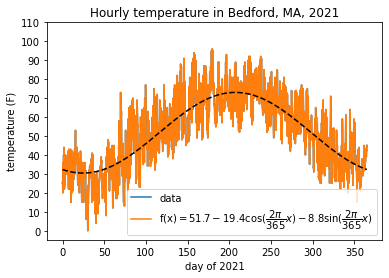
\includegraphics[width=0.45\linewidth]{img/C03weatherBedfordfit.png}
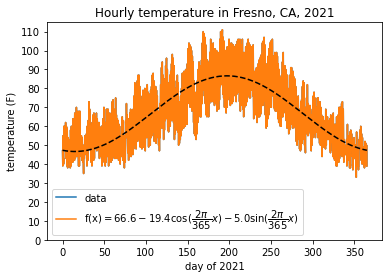
\includegraphics[width=0.45\linewidth]{img/C03weatherFresnofit.png}



\subsection{Normal equations}

\noindent\textbf{Choose parameters to minimize the error}
\begin{tcolorbox}
 With $A\vc{w} \approx \vc{y}$, the error is $\vc{e}(\vc{w}) = A\vc{w}-\vc{y}$, and the sum of squared errors is $E(\vc{w}) = \vc{e}(\vc{w})^T\vc{e}(\vc{w})$.
    
    The error function is a scalar function of $\vc{w}$.
\end{tcolorbox}
 To solve $A\vc{w} = \vc{y}$ in the least squares sense, find $\vc{w}$ that minimizes the error function, $E(\vc{w})$.
    
    i.e. Find $\vc{w}$ such that $\dfrac{dE(\vc{w})}{d\vc{w}} = 0$ (and check that $E$ is minimized at this point by examining second derivatives).  $\dfrac{dE(\vc{w})}{d\vc{w}}=\left[\begin{array}{ccc} \dfrac{\partial E}{\partial w_1} \hdots \dfrac{\partial E}{\partial w_M} \end{array}\right]$ is also denoted $DE(\vc{w})$, or simply $DE$.
    
    \emph{Notice that $DE$ is the transpose of $\nabla E$, the gradient of $E$}
    

Note: $\varphi_k(x)$ linearly independent means the columns of $A$ are also linearly independent.

% https://math.stackexchange.com/questions/834420/prove-that-ata-is-positive-definite


\begin{enumerate}[resume=classQ]
\item Let $E(\vc{w}) = w_1^2+4w_1w_2+3w_2^2+w_2$.  
 Find $\vc{w}^*$ so that $E(\vc{w}^*)$ is a critical point of the function $E$.
%\item Recall: $E(\vc{w}^*)$ may be a local minimum, local maximum, or saddle point.  



%\end{parts}

\end{enumerate}

\noindent\textbf{Classifying a critical point}
\begin{tcolorbox}
\begin{itemize}
\itemsep0pt
    \item At a critical point, $\vc{w}^*$, the derivative of the output, $\left[DE\right]_{\vc{w}^*} = \vc{0}$.  The critical point might be a local minimum, local maximum, or saddle point.
    \item We are looking for a local minimum, so we want $E(\vc{w}^*) < E(\vc{w}^*+\vc{h})$, where $\vc{h}$ is any small vector so $\vc{w}^*+\vc{h}$ is an input close to $\vc{w}^*$.
    
    \item Approximate $E$ at nearby points via Taylor expansion to determine whether $E(\vc{w}^*)$ is a local minimum:
    \[E(\vc{w}^*+\vc{h}) = E(\vc{w}^*) + \left[DE\right]_{\vc{w}^*}\vc{h} + \frac{1}{2} \vc{h}^T\left[D^2E\right]_{\vc{w}^*}\vc{h} + \mathcal{O}(\Vert\vc{h}\Vert^3)\]
    
        \end{itemize}
\end{tcolorbox}
    
    \begin{tcolorbox}
    \begin{itemize}
  \item  
    At the $\vc{w}^*$ the first derivative, $\left[DE\right]_{\vc{w}^*}$, is $\vc{0}$, so this simplifies to 
    
    \[E(\vc{w}^*+\vc{h}) = E(\vc{w}^*) +  \frac{1}{2} \vc{h}^T\left[D^2E\right]_{\vc{w}^*}\vc{h} + \mathcal{O}(\Vert\vc{h}\Vert^3)\]
    
    \item For the critical point to be a local minimum, we need $\vc{h}^T\left[D^2E\right]_{\vc{w}^*}\vc{h}>0$ for nonzero $\vc{h}$. 
    \end{itemize}
\end{tcolorbox}

\begin{tcolorbox}
    \begin{itemize}
    \item A symmetric matrix $M$ where $\vc{h}^TA\vc{h}>0$ for all nonzero $\vc{h}$ is called \textbf{positive definite}.
    
    A symmetric matrix $M$ is positive definite if and only if the eigenvalues of $M$ are positive.
  %  This will be true if the eigenvalues of $\left[D^2E\right]_{\vc{w}^*}$ are positive
    
    \item $\left[D^2E\right]_{\vc{w}^*} = \left[\begin{array}{ccc}
    \dfrac{\partial^2E}{\partial w_1 \partial w_1} & \hdots & \dfrac{\partial^2E}{\partial w_1 \partial w_M} \\
    \vdots & \ddots & \vdots \\
    
    \dfrac{\partial^2E}{\partial w_M \partial w_1} & \hdots & \dfrac{\partial^2E}{\partial w_M \partial w_M}
    \end{array}\right]$. This is the \textbf{Hessian} matrix.  The equality of mixed partials means that the Hessian matrix is symmetric.
    \item $\vc{w}^*$ will be a local minimum if the Hessian matrix, evaluated at $\vc{w}^*$, is positive definite.
\end{itemize}
\end{tcolorbox}
\begin{enumerate}[resume=classQ]
\item Let $E(\vc{w}) = w_1^2+4w_1w_2+3w_2^2+w_2$.  
 
 You found a critical point $(w_1, w_2)^*$ above.  
 \begin{parts}
\item  Now find the Hessian matrix, evaluated at this critical point.
\item The trace of a matrix gives the sum of the eigenvalues, $\lambda_1+\lambda_2$.  The determinant of a matrix gives the product of the eigenvalues, $\lambda_1\lambda_2$.  For a $2\times 2$ matrix this information is sufficient to determine the sign of the eigenvalues.  

Find the trace and determinant of the Hessian and determine the sign of the eigenvalues. 
 \end{parts}
 




%\end{parts}

\end{enumerate}

\noindent\textbf{The normal equations}
\begin{tcolorbox}
Setting $DE(\vc{w}) = \vc{0}$ will result in a matrix equation called the \textbf{normal equations}.  Solving the normal equations for $\vc{w}$ will allow us to find $\vc{w}^*$.
\end{tcolorbox}

\begin{align*}
        E(\vc{w}) &= \vc{e}^T\vc{e} \\
        &=(A\vc{w}-\vc{y})^T(A\vc{w}-\vc{y}) \\
        &=\left((A\vc{w})^T-\vc{y}^T\right)(A\vc{w}-\vc{y}) \\
        &=\left(\vc{w}^TA^T-\vc{y}^T\right)(A\vc{w}-\vc{y}) \\
        &=\left(\vc{w}^TA^T-\vc{y}^T\right)(A\vc{w}-\vc{y}) \\
        &=\vc{w}^TA^TA\vc{w}-\vc{w}^TA^T\vc{y}-\vc{y}^TA\vc{w} + \vc{y}^T\vc{y} \\
        &=\vc{w}^TA^TA\vc{w}-\vc{w}^TA^T\vc{y}-\vc{y}^TA\vc{w} + \vc{y}^T\vc{y}
    \end{align*}
    
\begin{tcolorbox}
    $E(\vc{w})$ is a scalar valued function, so $\vc{w}^TA^T\vc{y}$ is a scalar.  $\vc{w}^TA^T\vc{y}=(\vc{y}^TA\vc{w})^T$.  For a scalar, $x$, $x^T = x$ so $\vc{w}^TA^T\vc{y} = \vc{y}^TA\vc{w}$.  We have
    \[E(\vc{w}) = \vc{w}^TA^TA\vc{w}-2\vc{y}^TA\vc{w} + \vc{y}^T\vc{y}\]
    
To find $DE$ we will need some facts about matrix derivatives.
\begin{itemize}
\itemsep0pt
    \item $\left[D A\vc{x}\right] = A$.
    \item (product rule) $\left[D\left(\vc{u}^T\vc{v}\right)\right]= \vc{u}^T\left[D\vc{v}\right]+\vc{v}^T\left[D\vc{u}\right]$
\end{itemize}
\end{tcolorbox}

\begin{enumerate}[resume=classQ]
    \item Find the normal equations
    \begin{parts}
    \item Let $\vc{u} = A\vc{w}$ and use the product rule to show that $\left[DE\right] = -2\vc{y}^TA + 2\vc{w}^TA^TA$
    \item Set $\left[DE\right] = \vc{0}$ and rearrange to find \[A^TA\vc{w}=A^T\vc{y} \]
   These are the \textbf{normal equations}.
    \item Identify the dimensions of $A^TA$, $\vc{w}$, and $A^T\vc{y}$.
    \end{parts}
   
    
\end{enumerate}

\end{document}
